\documentclass[1p]{elsarticle_modified}
%\bibliographystyle{elsarticle-num}

%\usepackage[colorlinks]{hyperref}
%\usepackage{abbrmath_seonhwa} %\Abb, \Ascr, \Acal ,\Abf, \Afrak
\usepackage{amsfonts}
\usepackage{amssymb}
\usepackage{amsmath}
\usepackage{amsthm}
\usepackage{scalefnt}
\usepackage{amsbsy}
\usepackage{kotex}
\usepackage{caption}
\usepackage{subfig}
\usepackage{color}
\usepackage{graphicx}
\usepackage{xcolor} %% white, black, red, green, blue, cyan, magenta, yellow
\usepackage{float}
\usepackage{setspace}
\usepackage{hyperref}

\usepackage{tikz}
\usetikzlibrary{arrows}

\usepackage{multirow}
\usepackage{array} % fixed length table
\usepackage{hhline}

%%%%%%%%%%%%%%%%%%%%%
\makeatletter
\renewcommand*\env@matrix[1][\arraystretch]{%
	\edef\arraystretch{#1}%
	\hskip -\arraycolsep
	\let\@ifnextchar\new@ifnextchar
	\array{*\c@MaxMatrixCols c}}
\makeatother %https://tex.stackexchange.com/questions/14071/how-can-i-increase-the-line-spacing-in-a-matrix
%%%%%%%%%%%%%%%

\usepackage[normalem]{ulem}

\newcommand{\msout}[1]{\ifmmode\text{\sout{\ensuremath{#1}}}\else\sout{#1}\fi}
%SOURCE: \msout is \stkout macro in https://tex.stackexchange.com/questions/20609/strikeout-in-math-mode

\newcommand{\cancel}[1]{
	\ifmmode
	{\color{red}\msout{#1}}
	\else
	{\color{red}\sout{#1}}
	\fi
}

\newcommand{\add}[1]{
	{\color{blue}\uwave{#1}}
}

\newcommand{\replace}[2]{
	\ifmmode
	{\color{red}\msout{#1}}{\color{blue}\uwave{#2}}
	\else
	{\color{red}\sout{#1}}{\color{blue}\uwave{#2}}
	\fi
}

\newcommand{\Sol}{\mathcal{S}} %segment
\newcommand{\D}{D} %diagram
\newcommand{\A}{\mathcal{A}} %arc


%%%%%%%%%%%%%%%%%%%%%%%%%%%%%5 test

\def\sl{\operatorname{\textup{SL}}(2,\Cbb)}
\def\psl{\operatorname{\textup{PSL}}(2,\Cbb)}
\def\quan{\mkern 1mu \triangleright \mkern 1mu}

\theoremstyle{definition}
\newtheorem{thm}{Theorem}[section]
\newtheorem{prop}[thm]{Proposition}
\newtheorem{lem}[thm]{Lemma}
\newtheorem{ques}[thm]{Question}
\newtheorem{cor}[thm]{Corollary}
\newtheorem{defn}[thm]{Definition}
\newtheorem{exam}[thm]{Example}
\newtheorem{rmk}[thm]{Remark}
\newtheorem{alg}[thm]{Algorithm}

\newcommand{\I}{\sqrt{-1}}
\begin{document}

%\begin{frontmatter}
%
%\title{Boundary parabolic representations of knots up to 8 crossings}
%
%%% Group authors per affiliation:
%\author{Yunhi Cho} 
%\address{Department of Mathematics, University of Seoul, Seoul, Korea}
%\ead{yhcho@uos.ac.kr}
%
%
%\author{Seonhwa Kim} %\fnref{s_kim}}
%\address{Center for Geometry and Physics, Institute for Basic Science, Pohang, 37673, Korea}
%\ead{ryeona17@ibs.re.kr}
%
%\author{Hyuk Kim}
%\address{Department of Mathematical Sciences, Seoul National University, Seoul 08826, Korea}
%\ead{hyukkim@snu.ac.kr}
%
%\author{Seokbeom Yoon}
%\address{Department of Mathematical Sciences, Seoul National University, Seoul, 08826,  Korea}
%\ead{sbyoon15@snu.ac.kr}
%
%\begin{abstract}
%We find all boundary parabolic representation of knots up to 8 crossings.
%
%\end{abstract}
%\begin{keyword}
%    \MSC[2010] 57M25 
%\end{keyword}
%
%\end{frontmatter}

%\linenumbers
%\tableofcontents
%
\newcommand\colored[1]{\textcolor{white}{\rule[-0.35ex]{0.8em}{1.4ex}}\kern-0.8em\color{red} #1}%
%\newcommand\colored[1]{\textcolor{white}{ #1}\kern-2.17ex	\textcolor{white}{ #1}\kern-1.81ex	\textcolor{white}{ #1}\kern-2.15ex\color{red}#1	}

{\Large $\underline{12n_{0187}~(K12n_{0187})}$}

\setlength{\tabcolsep}{10pt}
\renewcommand{\arraystretch}{1.6}
\vspace{1cm}\begin{tabular}{m{100pt}>{\centering\arraybackslash}m{274pt}}
\multirow{5}{120pt}{
	\centering
	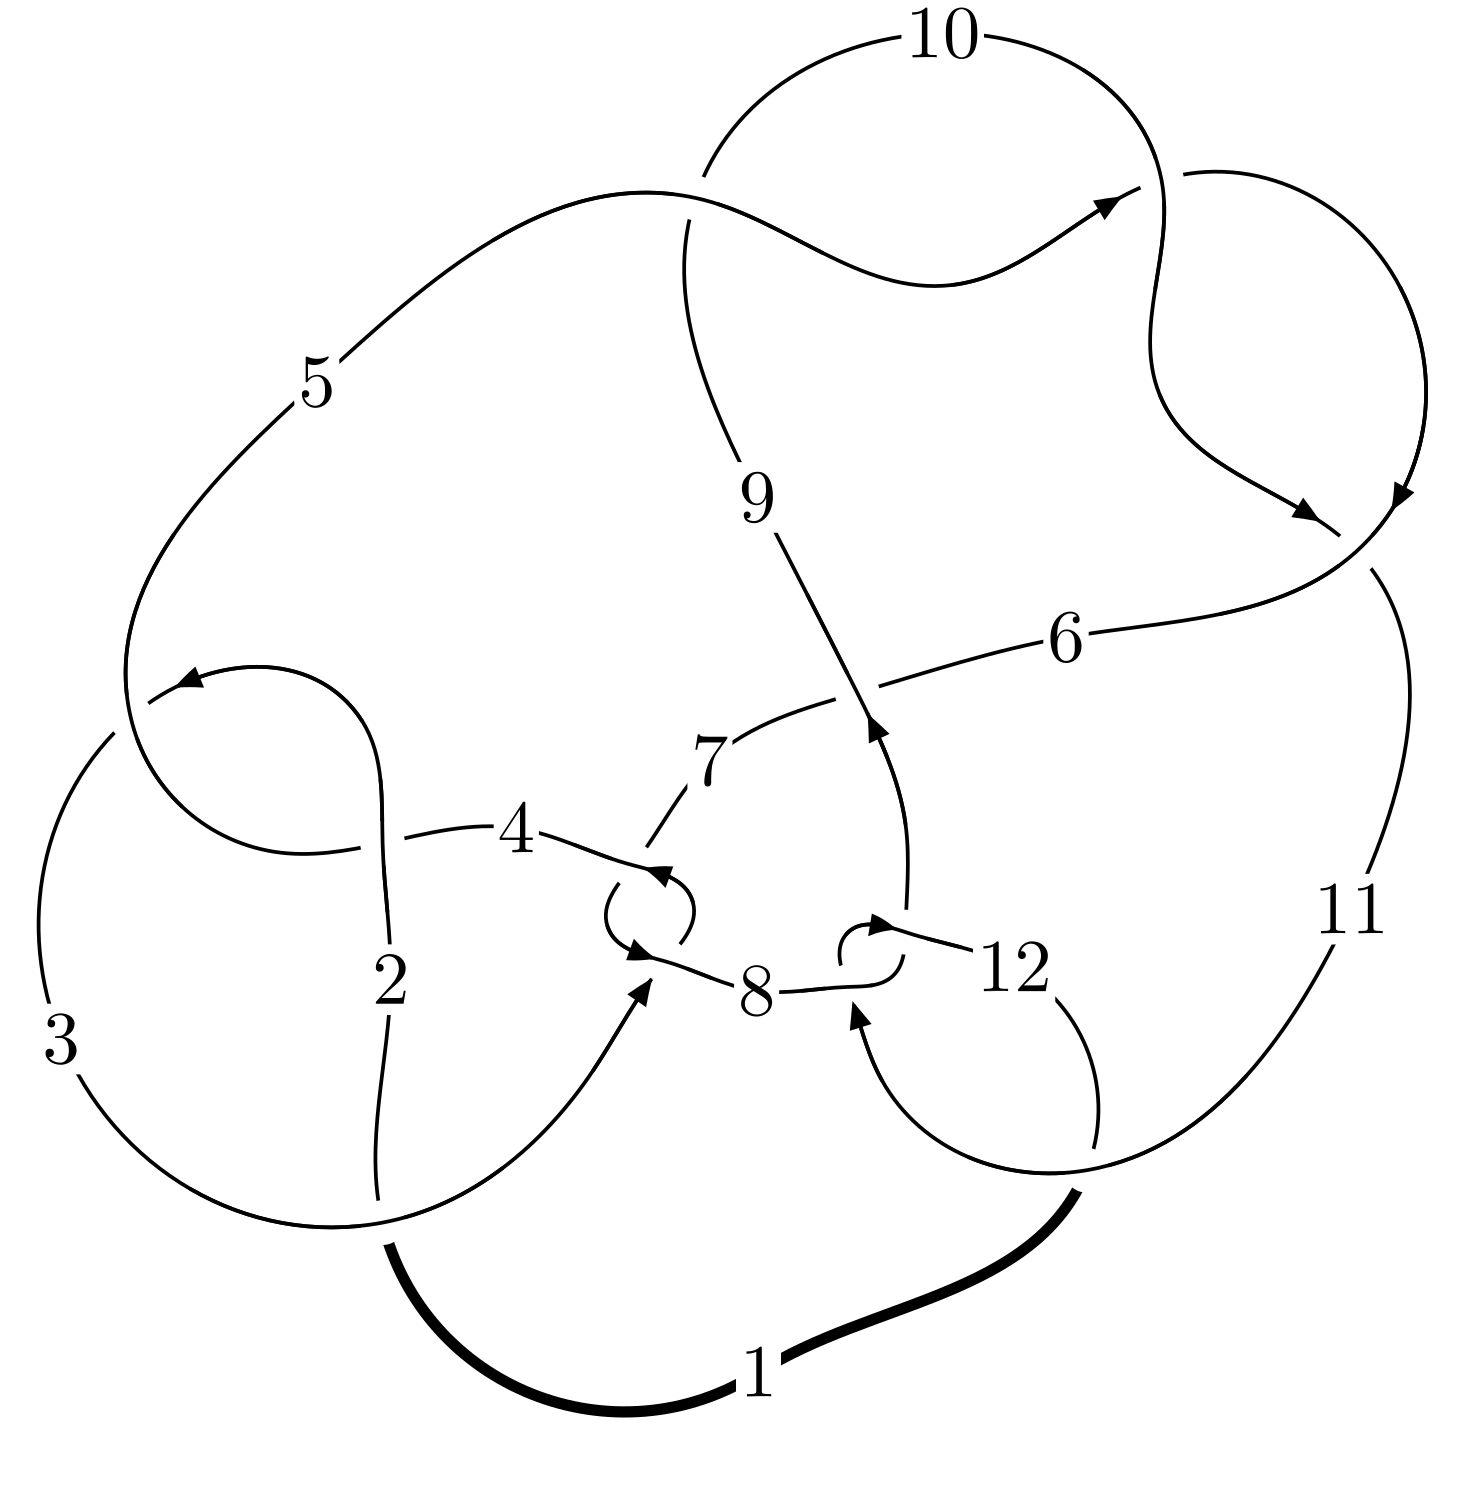
\includegraphics[width=112pt]{../../../GIT/diagram.site/Diagrams/png/2276_12n_0187.png}\\
\ \ \ A knot diagram\footnotemark}&
\allowdisplaybreaks
\textbf{Linearized knot diagam} \\
\cline{2-2}
 &
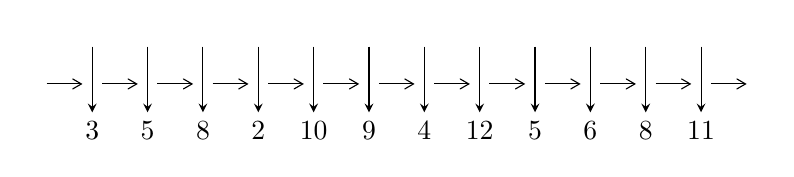
\begin{tikzpicture}[x=20pt, y=17pt]
	% nodes
	\node (C0) at (0, 0) {};
	\node (C1) at (1, 0) {};
	\node (C1U) at (1, +1) {};
	\node (C1D) at (1, -1) {3};

	\node (C2) at (2, 0) {};
	\node (C2U) at (2, +1) {};
	\node (C2D) at (2, -1) {5};

	\node (C3) at (3, 0) {};
	\node (C3U) at (3, +1) {};
	\node (C3D) at (3, -1) {8};

	\node (C4) at (4, 0) {};
	\node (C4U) at (4, +1) {};
	\node (C4D) at (4, -1) {2};

	\node (C5) at (5, 0) {};
	\node (C5U) at (5, +1) {};
	\node (C5D) at (5, -1) {10};

	\node (C6) at (6, 0) {};
	\node (C6U) at (6, +1) {};
	\node (C6D) at (6, -1) {9};

	\node (C7) at (7, 0) {};
	\node (C7U) at (7, +1) {};
	\node (C7D) at (7, -1) {4};

	\node (C8) at (8, 0) {};
	\node (C8U) at (8, +1) {};
	\node (C8D) at (8, -1) {12};

	\node (C9) at (9, 0) {};
	\node (C9U) at (9, +1) {};
	\node (C9D) at (9, -1) {5};

	\node (C10) at (10, 0) {};
	\node (C10U) at (10, +1) {};
	\node (C10D) at (10, -1) {6};

	\node (C11) at (11, 0) {};
	\node (C11U) at (11, +1) {};
	\node (C11D) at (11, -1) {8};

	\node (C12) at (12, 0) {};
	\node (C12U) at (12, +1) {};
	\node (C12D) at (12, -1) {11};
	\node (C13) at (13, 0) {};

	% arrows
	\draw[->,>={angle 60}]
	(C0) edge (C1) (C1) edge (C2) (C2) edge (C3) (C3) edge (C4) (C4) edge (C5) (C5) edge (C6) (C6) edge (C7) (C7) edge (C8) (C8) edge (C9) (C9) edge (C10) (C10) edge (C11) (C11) edge (C12) (C12) edge (C13) ;	\draw[->,>=stealth]
	(C1U) edge (C1D) (C2U) edge (C2D) (C3U) edge (C3D) (C4U) edge (C4D) (C5U) edge (C5D) (C6U) edge (C6D) (C7U) edge (C7D) (C8U) edge (C8D) (C9U) edge (C9D) (C10U) edge (C10D) (C11U) edge (C11D) (C12U) edge (C12D) ;
	\end{tikzpicture} \\
\hhline{~~} \\& 
\textbf{Solving Sequence} \\ \cline{2-2} 
 &
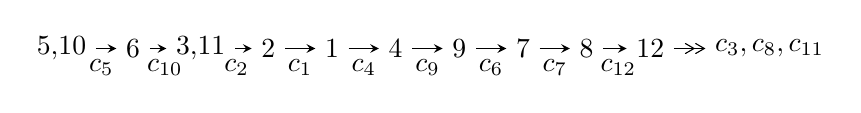
\begin{tikzpicture}[x=23pt, y=7pt]
	% node
	\node (A0) at (-1/8, 0) {5,10};
	\node (A1) at (1, 0) {6};
	\node (A2) at (33/16, 0) {3,11};
	\node (A3) at (25/8, 0) {2};
	\node (A4) at (33/8, 0) {1};
	\node (A5) at (41/8, 0) {4};
	\node (A6) at (49/8, 0) {9};
	\node (A7) at (57/8, 0) {7};
	\node (A8) at (65/8, 0) {8};
	\node (A9) at (73/8, 0) {12};
	\node (C1) at (1/2, -1) {$c_{5}$};
	\node (C2) at (3/2, -1) {$c_{10}$};
	\node (C3) at (21/8, -1) {$c_{2}$};
	\node (C4) at (29/8, -1) {$c_{1}$};
	\node (C5) at (37/8, -1) {$c_{4}$};
	\node (C6) at (45/8, -1) {$c_{9}$};
	\node (C7) at (53/8, -1) {$c_{6}$};
	\node (C8) at (61/8, -1) {$c_{7}$};
	\node (C9) at (69/8, -1) {$c_{12}$};
	\node (A10) at (11, 0) {$c_{3},c_{8},c_{11}$};

	% edge
	\draw[->,>=stealth]	
	(A0) edge (A1) (A1) edge (A2) (A2) edge (A3) (A3) edge (A4) (A4) edge (A5) (A5) edge (A6) (A6) edge (A7) (A7) edge (A8) (A8) edge (A9) ;
	\draw[->>,>={angle 60}]	
	(A9) edge (A10);
\end{tikzpicture} \\ 

\end{tabular} \\

\footnotetext{
The image of knot diagram is generated by the software ``\textbf{Draw programme}" developed by Andrew Bartholomew(\url{http://www.layer8.co.uk/maths/draw/index.htm\#Running-draw}), where we modified some parts for our purpose(\url{https://github.com/CATsTAILs/LinksPainter}).
}\phantom \\ \newline 
\centering \textbf{Ideals for irreducible components\footnotemark of $X_{\text{par}}$} 
 
\begin{align*}
I^u_{1}&=\langle 
-4.64866\times10^{37} u^{39}-3.95589\times10^{37} u^{38}+\cdots+1.60462\times10^{38} b-1.99553\times10^{38},\\
\phantom{I^u_{1}}&\phantom{= \langle  }1.25972\times10^{38} u^{39}+6.09841\times10^{37} u^{38}+\cdots+3.20923\times10^{38} a+1.75553\times10^{39},\;u^{40}+2 u^{39}+\cdots+24 u+8\rangle \\
I^u_{2}&=\langle 
b+1,\;2 u^7+u^6-5 u^5-2 u^4+3 u^3+a+2 u+2,\;u^8+u^7-3 u^6-2 u^5+3 u^4+2 u-1\rangle \\
I^u_{3}&=\langle 
2 a^2-2 a u+b-4 a+2 u+2,\;4 a^3-6 a^2 u-12 a^2+12 a u+16 a-7 u-8,\;u^2-2\rangle \\
\\
I^v_{1}&=\langle 
a,\;- v^2+b-3 v+1,\;v^3+2 v^2-3 v+1\rangle \\
\end{align*}
\raggedright * 4 irreducible components of $\dim_{\mathbb{C}}=0$, with total 57 representations.\\
\footnotetext{All coefficients of polynomials are rational numbers. But the coefficients are sometimes approximated in decimal forms when there is not enough margin.}
\newpage
\renewcommand{\arraystretch}{1}
\centering \section*{I. $I^u_{1}= \langle -4.65\times10^{37} u^{39}-3.96\times10^{37} u^{38}+\cdots+1.60\times10^{38} b-2.00\times10^{38},\;1.26\times10^{38} u^{39}+6.10\times10^{37} u^{38}+\cdots+3.21\times10^{38} a+1.76\times10^{39},\;u^{40}+2 u^{39}+\cdots+24 u+8 \rangle$}
\flushleft \textbf{(i) Arc colorings}\\
\begin{tabular}{m{7pt} m{180pt} m{7pt} m{180pt} }
\flushright $a_{5}=$&$\begin{pmatrix}1\\0\end{pmatrix}$ \\
\flushright $a_{10}=$&$\begin{pmatrix}0\\u\end{pmatrix}$ \\
\flushright $a_{6}=$&$\begin{pmatrix}1\\u^2\end{pmatrix}$ \\
\flushright $a_{3}=$&$\begin{pmatrix}-0.392531 u^{39}-0.190027 u^{38}+\cdots-31.7178 u-5.47024\\0.289705 u^{39}+0.246532 u^{38}+\cdots+3.47362 u+1.24362\end{pmatrix}$ \\
\flushright $a_{11}=$&$\begin{pmatrix}- u\\- u^3+u\end{pmatrix}$ \\
\flushright $a_{2}=$&$\begin{pmatrix}-0.102825 u^{39}+0.0565047 u^{38}+\cdots-28.2442 u-4.22662\\0.289705 u^{39}+0.246532 u^{38}+\cdots+3.47362 u+1.24362\end{pmatrix}$ \\
\flushright $a_{1}=$&$\begin{pmatrix}0.0112960 u^{39}+0.165138 u^{38}+\cdots-6.59349 u+0.402568\\-0.409908 u^{39}-0.550903 u^{38}+\cdots-7.68190 u-4.87982\end{pmatrix}$ \\
\flushright $a_{4}=$&$\begin{pmatrix}-0.356445 u^{39}-0.0512403 u^{38}+\cdots-27.2073 u-3.79706\\-0.499643 u^{39}-0.495583 u^{38}+\cdots-9.08353 u-4.38695\end{pmatrix}$ \\
\flushright $a_{9}=$&$\begin{pmatrix}u\\u\end{pmatrix}$ \\
\flushright $a_{7}=$&$\begin{pmatrix}- u^4+u^2+1\\- u^4+2 u^2\end{pmatrix}$ \\
\flushright $a_{8}=$&$\begin{pmatrix}-0.0519172 u^{39}+0.0642471 u^{38}+\cdots-8.35273 u-0.669722\\0.130286 u^{39}+0.294618 u^{38}+\cdots+2.41118 u+2.66716\end{pmatrix}$ \\
\flushright $a_{12}=$&$\begin{pmatrix}-0.0519172 u^{39}+0.0642471 u^{38}+\cdots-8.35273 u-0.669722\\-0.358582 u^{39}-0.442506 u^{38}+\cdots-6.02980 u-4.01181\end{pmatrix}$\\&\end{tabular}
\flushleft \textbf{(ii) Obstruction class $= -1$}\\~\\
\flushleft \textbf{(iii) Cusp Shapes $= 6.32861 u^{39}+4.79660 u^{38}+\cdots+0.992255 u+10.7532$}\\~\\
\newpage\renewcommand{\arraystretch}{1}
\flushleft \textbf{(iv) u-Polynomials at the component}\newline \\
\begin{tabular}{m{50pt}|m{274pt}}
Crossings & \hspace{64pt}u-Polynomials at each crossing \\
\hline $$\begin{aligned}c_{1}\end{aligned}$$&$\begin{aligned}
&u^{40}+4 u^{39}+\cdots+2 u+1
\end{aligned}$\\
\hline $$\begin{aligned}c_{2},c_{4}\end{aligned}$$&$\begin{aligned}
&u^{40}-12 u^{39}+\cdots+2 u+1
\end{aligned}$\\
\hline $$\begin{aligned}c_{3},c_{7}\end{aligned}$$&$\begin{aligned}
&u^{40}+2 u^{39}+\cdots+1408 u-256
\end{aligned}$\\
\hline $$\begin{aligned}c_{5},c_{9},c_{10}\end{aligned}$$&$\begin{aligned}
&u^{40}+2 u^{39}+\cdots+24 u+8
\end{aligned}$\\
\hline $$\begin{aligned}c_{6}\end{aligned}$$&$\begin{aligned}
&u^{40}-6 u^{39}+\cdots+4248 u+1192
\end{aligned}$\\
\hline $$\begin{aligned}c_{8},c_{11}\end{aligned}$$&$\begin{aligned}
&u^{40}+5 u^{39}+\cdots+49 u+7
\end{aligned}$\\
\hline $$\begin{aligned}c_{12}\end{aligned}$$&$\begin{aligned}
&u^{40}+9 u^{39}+\cdots-63 u+49
\end{aligned}$\\
\hline
\end{tabular}\\~\\
\newpage\renewcommand{\arraystretch}{1}
\flushleft \textbf{(v) Riley Polynomials at the component}\newline \\
\begin{tabular}{m{50pt}|m{274pt}}
Crossings & \hspace{64pt}Riley Polynomials at each crossing \\
\hline $$\begin{aligned}c_{1}\end{aligned}$$&$\begin{aligned}
&y^{40}+76 y^{39}+\cdots-2330 y+1
\end{aligned}$\\
\hline $$\begin{aligned}c_{2},c_{4}\end{aligned}$$&$\begin{aligned}
&y^{40}-4 y^{39}+\cdots-2 y+1
\end{aligned}$\\
\hline $$\begin{aligned}c_{3},c_{7}\end{aligned}$$&$\begin{aligned}
&y^{40}+60 y^{39}+\cdots-4636672 y+65536
\end{aligned}$\\
\hline $$\begin{aligned}c_{5},c_{9},c_{10}\end{aligned}$$&$\begin{aligned}
&y^{40}-32 y^{39}+\cdots-1728 y+64
\end{aligned}$\\
\hline $$\begin{aligned}c_{6}\end{aligned}$$&$\begin{aligned}
&y^{40}+64 y^{39}+\cdots-52489536 y+1420864
\end{aligned}$\\
\hline $$\begin{aligned}c_{8},c_{11}\end{aligned}$$&$\begin{aligned}
&y^{40}-9 y^{39}+\cdots+63 y+49
\end{aligned}$\\
\hline $$\begin{aligned}c_{12}\end{aligned}$$&$\begin{aligned}
&y^{40}+55 y^{39}+\cdots-206241 y+2401
\end{aligned}$\\
\hline
\end{tabular}\\~\\
\newpage\flushleft \textbf{(vi) Complex Volumes and Cusp Shapes}
$$\begin{array}{c|c|c}  
\text{Solutions to }I^u_{1}& \I (\text{vol} + \sqrt{-1}CS) & \text{Cusp shape}\\
 \hline 
\begin{aligned}
u &= \phantom{-}0.897120 + 0.222335 I \\
a &= -1.274740 - 0.263007 I \\
b &= -1.187560 + 0.291372 I\end{aligned}
 & -3.03578 - 0.99249 I & -14.4826 + 4.2079 I \\ \hline\begin{aligned}
u &= \phantom{-}0.897120 - 0.222335 I \\
a &= -1.274740 + 0.263007 I \\
b &= -1.187560 - 0.291372 I\end{aligned}
 & -3.03578 + 0.99249 I & -14.4826 - 4.2079 I \\ \hline\begin{aligned}
u &= -0.771034 + 0.454110 I \\
a &= -0.157593 - 0.131539 I \\
b &= \phantom{-}0.140691 + 0.765731 I\end{aligned}
 & \phantom{-}0.072412 - 0.256498 I & -11.04074 - 0.73471 I \\ \hline\begin{aligned}
u &= -0.771034 - 0.454110 I \\
a &= -0.157593 + 0.131539 I \\
b &= \phantom{-}0.140691 - 0.765731 I\end{aligned}
 & \phantom{-}0.072412 + 0.256498 I & -11.04074 + 0.73471 I \\ \hline\begin{aligned}
u &= \phantom{-}0.215830 + 1.094140 I \\
a &= -0.14903 - 1.49112 I \\
b &= \phantom{-}1.21980 + 1.09723 I\end{aligned}
 & \phantom{-}13.1415 - 8.3613 I & -10.09689 + 4.44612 I \\ \hline\begin{aligned}
u &= \phantom{-}0.215830 - 1.094140 I \\
a &= -0.14903 + 1.49112 I \\
b &= \phantom{-}1.21980 - 1.09723 I\end{aligned}
 & \phantom{-}13.1415 + 8.3613 I & -10.09689 - 4.44612 I \\ \hline\begin{aligned}
u &= \phantom{-}0.214868 + 0.849389 I \\
a &= \phantom{-}0.456922 - 1.112210 I \\
b &= \phantom{-}0.092951 + 0.975052 I\end{aligned}
 & \phantom{-}3.63859 + 0.81418 I & -7.43543 - 0.73577 I \\ \hline\begin{aligned}
u &= \phantom{-}0.214868 - 0.849389 I \\
a &= \phantom{-}0.456922 + 1.112210 I \\
b &= \phantom{-}0.092951 - 0.975052 I\end{aligned}
 & \phantom{-}3.63859 - 0.81418 I & -7.43543 + 0.73577 I \\ \hline\begin{aligned}
u &= -1.068280 + 0.375203 I \\
a &= -1.15584 - 1.32730 I \\
b &= -1.241440 + 0.388080 I\end{aligned}
 & -2.92773 + 3.67752 I & -14.1570 - 3.8873 I \\ \hline\begin{aligned}
u &= -1.068280 - 0.375203 I \\
a &= -1.15584 + 1.32730 I \\
b &= -1.241440 - 0.388080 I\end{aligned}
 & -2.92773 - 3.67752 I & -14.1570 + 3.8873 I\\
 \hline 
 \end{array}$$\newpage$$\begin{array}{c|c|c}  
\text{Solutions to }I^u_{1}& \I (\text{vol} + \sqrt{-1}CS) & \text{Cusp shape}\\
 \hline 
\begin{aligned}
u &= \phantom{-}0.055954 + 1.139480 I \\
a &= -0.510868 + 1.235600 I \\
b &= \phantom{-}1.05505 - 1.26055 I\end{aligned}
 & \phantom{-}13.77200 + 0.23648 I & -9.35233 + 0.10077 I \\ \hline\begin{aligned}
u &= \phantom{-}0.055954 - 1.139480 I \\
a &= -0.510868 - 1.235600 I \\
b &= \phantom{-}1.05505 + 1.26055 I\end{aligned}
 & \phantom{-}13.77200 - 0.23648 I & -9.35233 - 0.10077 I \\ \hline\begin{aligned}
u &= -0.834687 + 0.181028 I \\
a &= \phantom{-}0.008249 + 1.189290 I \\
b &= \phantom{-}0.893530 - 0.929162 I\end{aligned}
 & \phantom{-}0.56575 + 3.31942 I & -15.0343 - 3.7698 I \\ \hline\begin{aligned}
u &= -0.834687 - 0.181028 I \\
a &= \phantom{-}0.008249 - 1.189290 I \\
b &= \phantom{-}0.893530 + 0.929162 I\end{aligned}
 & \phantom{-}0.56575 - 3.31942 I & -15.0343 + 3.7698 I \\ \hline\begin{aligned}
u &= -1.298310 + 0.059006 I \\
a &= \phantom{-}1.144330 + 0.058961 I \\
b &= \phantom{-}0.832938 - 0.605919 I\end{aligned}
 & -1.84528 + 2.59969 I & -12.00000 - 2.54541 I \\ \hline\begin{aligned}
u &= -1.298310 - 0.059006 I \\
a &= \phantom{-}1.144330 - 0.058961 I \\
b &= \phantom{-}0.832938 + 0.605919 I\end{aligned}
 & -1.84528 - 2.59969 I & -12.00000 + 2.54541 I \\ \hline\begin{aligned}
u &= \phantom{-}1.212760 + 0.510150 I \\
a &= -0.356611 + 0.737488 I \\
b &= -0.343875 - 1.008720 I\end{aligned}
 & \phantom{-}0.58084 - 5.79218 I & -12.00000 + 5.32251 I \\ \hline\begin{aligned}
u &= \phantom{-}1.212760 - 0.510150 I \\
a &= -0.356611 - 0.737488 I \\
b &= -0.343875 + 1.008720 I\end{aligned}
 & \phantom{-}0.58084 + 5.79218 I & -12.00000 - 5.32251 I \\ \hline\begin{aligned}
u &= \phantom{-}1.341590 + 0.066077 I \\
a &= \phantom{-}1.157320 - 0.440885 I \\
b &= \phantom{-}0.011549 + 0.213669 I\end{aligned}
 & -6.40298 - 0.09411 I & -12.00000 + 0. I\phantom{ +0.000000I} \\ \hline\begin{aligned}
u &= \phantom{-}1.341590 - 0.066077 I \\
a &= \phantom{-}1.157320 + 0.440885 I \\
b &= \phantom{-}0.011549 - 0.213669 I\end{aligned}
 & -6.40298 + 0.09411 I & -12.00000 + 0. I\phantom{ +0.000000I}\\
 \hline 
 \end{array}$$\newpage$$\begin{array}{c|c|c}  
\text{Solutions to }I^u_{1}& \I (\text{vol} + \sqrt{-1}CS) & \text{Cusp shape}\\
 \hline 
\begin{aligned}
u &= \phantom{-}1.344310 + 0.274263 I \\
a &= \phantom{-}1.203800 - 0.373288 I \\
b &= \phantom{-}0.758510 + 0.290373 I\end{aligned}
 & -3.47032 - 7.09799 I & \phantom{-0.000000 } 0 \\ \hline\begin{aligned}
u &= \phantom{-}1.344310 - 0.274263 I \\
a &= \phantom{-}1.203800 + 0.373288 I \\
b &= \phantom{-}0.758510 - 0.290373 I\end{aligned}
 & -3.47032 + 7.09799 I & \phantom{-0.000000 } 0 \\ \hline\begin{aligned}
u &= -0.187892 + 0.587668 I \\
a &= \phantom{-}0.380383 + 0.661515 I \\
b &= \phantom{-}0.724223 - 0.526726 I\end{aligned}
 & \phantom{-}1.29420 + 3.83935 I & -7.67979 - 8.27282 I \\ \hline\begin{aligned}
u &= -0.187892 - 0.587668 I \\
a &= \phantom{-}0.380383 - 0.661515 I \\
b &= \phantom{-}0.724223 + 0.526726 I\end{aligned}
 & \phantom{-}1.29420 - 3.83935 I & -7.67979 + 8.27282 I \\ \hline\begin{aligned}
u &= -1.40352\phantom{ +0.000000I} \\
a &= \phantom{-}13.1227\phantom{ +0.000000I} \\
b &= -0.992359\phantom{ +0.000000I}\end{aligned}
 & -8.20369\phantom{ +0.000000I} & -295.210\phantom{ +0.000000I} \\ \hline\begin{aligned}
u &= \phantom{-}1.217640 + 0.701085 I \\
a &= -0.398099 + 0.182880 I \\
b &= \phantom{-}1.08177 - 1.20718 I\end{aligned}
 & \phantom{-}10.13750 + 2.10810 I & \phantom{-0.000000 } 0 \\ \hline\begin{aligned}
u &= \phantom{-}1.217640 - 0.701085 I \\
a &= -0.398099 - 0.182880 I \\
b &= \phantom{-}1.08177 + 1.20718 I\end{aligned}
 & \phantom{-}10.13750 - 2.10810 I & \phantom{-0.000000 } 0 \\ \hline\begin{aligned}
u &= -1.41252 + 0.12831 I \\
a &= \phantom{-}0.979228 + 0.146823 I \\
b &= \phantom{-}0.678609 - 0.746967 I\end{aligned}
 & -1.77463 + 2.63558 I & \phantom{-0.000000 } 0 \\ \hline\begin{aligned}
u &= -1.41252 - 0.12831 I \\
a &= \phantom{-}0.979228 - 0.146823 I \\
b &= \phantom{-}0.678609 + 0.746967 I\end{aligned}
 & -1.77463 - 2.63558 I & \phantom{-0.000000 } 0 \\ \hline\begin{aligned}
u &= \phantom{-}1.46431\phantom{ +0.000000I} \\
a &= \phantom{-}0.581453\phantom{ +0.000000I} \\
b &= -0.422164\phantom{ +0.000000I}\end{aligned}
 & -6.89614\phantom{ +0.000000I} & \phantom{-0.000000 } 0\\
 \hline 
 \end{array}$$\newpage$$\begin{array}{c|c|c}  
\text{Solutions to }I^u_{1}& \I (\text{vol} + \sqrt{-1}CS) & \text{Cusp shape}\\
 \hline 
\begin{aligned}
u &= \phantom{-}1.35026 + 0.61000 I \\
a &= \phantom{-}0.81792 - 1.16224 I \\
b &= \phantom{-}1.17901 + 1.12040 I\end{aligned}
 & \phantom{-}9.78004 - 6.39860 I & \phantom{-0.000000 } 0 \\ \hline\begin{aligned}
u &= \phantom{-}1.35026 - 0.61000 I \\
a &= \phantom{-}0.81792 + 1.16224 I \\
b &= \phantom{-}1.17901 - 1.12040 I\end{aligned}
 & \phantom{-}9.78004 + 6.39860 I & \phantom{-0.000000 } 0 \\ \hline\begin{aligned}
u &= -0.314968 + 0.399432 I \\
a &= \phantom{-}1.012740 + 0.763059 I \\
b &= -0.781356 - 0.355549 I\end{aligned}
 & -0.815291 - 0.298544 I & -10.56718 - 0.99043 I \\ \hline\begin{aligned}
u &= -0.314968 - 0.399432 I \\
a &= \phantom{-}1.012740 - 0.763059 I \\
b &= -0.781356 + 0.355549 I\end{aligned}
 & -0.815291 + 0.298544 I & -10.56718 + 0.99043 I \\ \hline\begin{aligned}
u &= -1.42513 + 0.56145 I \\
a &= -0.492105 - 0.012487 I \\
b &= \phantom{-}0.86996 + 1.29131 I\end{aligned}
 & \phantom{-}9.15481 + 5.80967 I & \phantom{-0.000000 } 0 \\ \hline\begin{aligned}
u &= -1.42513 - 0.56145 I \\
a &= -0.492105 + 0.012487 I \\
b &= \phantom{-}0.86996 - 1.29131 I\end{aligned}
 & \phantom{-}9.15481 - 5.80967 I & \phantom{-0.000000 } 0 \\ \hline\begin{aligned}
u &= -1.47346 + 0.47082 I \\
a &= \phantom{-}1.11672 + 1.20821 I \\
b &= \phantom{-}1.24799 - 0.96895 I\end{aligned}
 & \phantom{-}7.7860 + 13.9558 I & \phantom{-0.000000 } 0 \\ \hline\begin{aligned}
u &= -1.47346 - 0.47082 I \\
a &= \phantom{-}1.11672 - 1.20821 I \\
b &= \phantom{-}1.24799 + 0.96895 I\end{aligned}
 & \phantom{-}7.7860 - 13.9558 I & \phantom{-0.000000 } 0 \\ \hline\begin{aligned}
u &= -0.427942\phantom{ +0.000000I} \\
a &= \phantom{-}0.826467\phantom{ +0.000000I} \\
b &= -0.164518\phantom{ +0.000000I}\end{aligned}
 & -0.684223\phantom{ +0.000000I} & -14.1610\phantom{ +0.000000I} \\ \hline\begin{aligned}
u &= \phantom{-}0.239037\phantom{ +0.000000I} \\
a &= -13.0961\phantom{ +0.000000I} \\
b &= -0.885633\phantom{ +0.000000I}\end{aligned}
 & -2.91744\phantom{ +0.000000I} & -60.2580\phantom{ +0.000000I}\\
 \hline 
 \end{array}$$\newpage\newpage\renewcommand{\arraystretch}{1}
\centering \section*{II. $I^u_{2}= \langle b+1,\;2 u^7+u^6-5 u^5-2 u^4+3 u^3+a+2 u+2,\;u^8+u^7-3 u^6-2 u^5+3 u^4+2 u-1 \rangle$}
\flushleft \textbf{(i) Arc colorings}\\
\begin{tabular}{m{7pt} m{180pt} m{7pt} m{180pt} }
\flushright $a_{5}=$&$\begin{pmatrix}1\\0\end{pmatrix}$ \\
\flushright $a_{10}=$&$\begin{pmatrix}0\\u\end{pmatrix}$ \\
\flushright $a_{6}=$&$\begin{pmatrix}1\\u^2\end{pmatrix}$ \\
\flushright $a_{3}=$&$\begin{pmatrix}-2 u^7- u^6+5 u^5+2 u^4-3 u^3-2 u-2\\-1\end{pmatrix}$ \\
\flushright $a_{11}=$&$\begin{pmatrix}- u\\- u^3+u\end{pmatrix}$ \\
\flushright $a_{2}=$&$\begin{pmatrix}-2 u^7- u^6+5 u^5+2 u^4-3 u^3-2 u-3\\-1\end{pmatrix}$ \\
\flushright $a_{1}=$&$\begin{pmatrix}-1\\0\end{pmatrix}$ \\
\flushright $a_{4}=$&$\begin{pmatrix}-2 u^7- u^6+5 u^5+2 u^4-3 u^3-2 u-2\\-1\end{pmatrix}$ \\
\flushright $a_{9}=$&$\begin{pmatrix}u\\u\end{pmatrix}$ \\
\flushright $a_{7}=$&$\begin{pmatrix}- u^4+u^2+1\\- u^4+2 u^2\end{pmatrix}$ \\
\flushright $a_{8}=$&$\begin{pmatrix}- u^4+u^2+1\\- u^4+2 u^2\end{pmatrix}$ \\
\flushright $a_{12}=$&$\begin{pmatrix}u^4- u^2-1\\u^6-2 u^4+u^2\end{pmatrix}$\\&\end{tabular}
\flushleft \textbf{(ii) Obstruction class $= 1$}\\~\\
\flushleft \textbf{(iii) Cusp Shapes $= -4 u^7+u^6+10 u^5-3 u^4-6 u^3+2 u^2-4 u-11$}\\~\\
\newpage\renewcommand{\arraystretch}{1}
\flushleft \textbf{(iv) u-Polynomials at the component}\newline \\
\begin{tabular}{m{50pt}|m{274pt}}
Crossings & \hspace{64pt}u-Polynomials at each crossing \\
\hline $$\begin{aligned}c_{1},c_{2}\end{aligned}$$&$\begin{aligned}
&(u-1)^8
\end{aligned}$\\
\hline $$\begin{aligned}c_{3},c_{7}\end{aligned}$$&$\begin{aligned}
&u^8
\end{aligned}$\\
\hline $$\begin{aligned}c_{4}\end{aligned}$$&$\begin{aligned}
&(u+1)^8
\end{aligned}$\\
\hline $$\begin{aligned}c_{5}\end{aligned}$$&$\begin{aligned}
&u^8+u^7-3 u^6-2 u^5+3 u^4+2 u-1
\end{aligned}$\\
\hline $$\begin{aligned}c_{6}\end{aligned}$$&$\begin{aligned}
&u^8-3 u^7+7 u^6-10 u^5+11 u^4-10 u^3+6 u^2-4 u+1
\end{aligned}$\\
\hline $$\begin{aligned}c_{8}\end{aligned}$$&$\begin{aligned}
&u^8- u^7- u^6+2 u^5+u^4-2 u^3+2 u-1
\end{aligned}$\\
\hline $$\begin{aligned}c_{9},c_{10}\end{aligned}$$&$\begin{aligned}
&u^8- u^7-3 u^6+2 u^5+3 u^4-2 u-1
\end{aligned}$\\
\hline $$\begin{aligned}c_{11}\end{aligned}$$&$\begin{aligned}
&u^8+u^7- u^6-2 u^5+u^4+2 u^3-2 u-1
\end{aligned}$\\
\hline $$\begin{aligned}c_{12}\end{aligned}$$&$\begin{aligned}
&u^8+3 u^7+7 u^6+10 u^5+11 u^4+10 u^3+6 u^2+4 u+1
\end{aligned}$\\
\hline
\end{tabular}\\~\\
\newpage\renewcommand{\arraystretch}{1}
\flushleft \textbf{(v) Riley Polynomials at the component}\newline \\
\begin{tabular}{m{50pt}|m{274pt}}
Crossings & \hspace{64pt}Riley Polynomials at each crossing \\
\hline $$\begin{aligned}c_{1},c_{2},c_{4}\end{aligned}$$&$\begin{aligned}
&(y-1)^8
\end{aligned}$\\
\hline $$\begin{aligned}c_{3},c_{7}\end{aligned}$$&$\begin{aligned}
&y^8
\end{aligned}$\\
\hline $$\begin{aligned}c_{5},c_{9},c_{10}\end{aligned}$$&$\begin{aligned}
&y^8-7 y^7+19 y^6-22 y^5+3 y^4+14 y^3-6 y^2-4 y+1
\end{aligned}$\\
\hline $$\begin{aligned}c_{6},c_{12}\end{aligned}$$&$\begin{aligned}
&y^8+5 y^7+11 y^6+6 y^5-17 y^4-34 y^3-22 y^2-4 y+1
\end{aligned}$\\
\hline $$\begin{aligned}c_{8},c_{11}\end{aligned}$$&$\begin{aligned}
&y^8-3 y^7+7 y^6-10 y^5+11 y^4-10 y^3+6 y^2-4 y+1
\end{aligned}$\\
\hline
\end{tabular}\\~\\
\newpage\flushleft \textbf{(vi) Complex Volumes and Cusp Shapes}
$$\begin{array}{c|c|c}  
\text{Solutions to }I^u_{2}& \I (\text{vol} + \sqrt{-1}CS) & \text{Cusp shape}\\
 \hline 
\begin{aligned}
u &= \phantom{-}1.180120 + 0.268597 I \\
a &= -0.914310 + 0.514779 I \\
b &= -1.00000\phantom{ +0.000000I}\end{aligned}
 & -2.68559 - 1.13123 I & -13.44913 - 0.23763 I \\ \hline\begin{aligned}
u &= \phantom{-}1.180120 - 0.268597 I \\
a &= -0.914310 - 0.514779 I \\
b &= -1.00000\phantom{ +0.000000I}\end{aligned}
 & -2.68559 + 1.13123 I & -13.44913 + 0.23763 I \\ \hline\begin{aligned}
u &= \phantom{-}0.108090 + 0.747508 I \\
a &= \phantom{-}0.036111 + 0.260696 I \\
b &= -1.00000\phantom{ +0.000000I}\end{aligned}
 & \phantom{-}0.51448 - 2.57849 I & -10.29693 + 2.50491 I \\ \hline\begin{aligned}
u &= \phantom{-}0.108090 - 0.747508 I \\
a &= \phantom{-}0.036111 - 0.260696 I \\
b &= -1.00000\phantom{ +0.000000I}\end{aligned}
 & \phantom{-}0.51448 + 2.57849 I & -10.29693 - 2.50491 I \\ \hline\begin{aligned}
u &= -1.37100\phantom{ +0.000000I} \\
a &= \phantom{-}2.88842\phantom{ +0.000000I} \\
b &= -1.00000\phantom{ +0.000000I}\end{aligned}
 & -8.14766\phantom{ +0.000000I} & -2.27260\phantom{ +0.000000I} \\ \hline\begin{aligned}
u &= -1.334530 + 0.318930 I \\
a &= -1.043070 - 0.634428 I \\
b &= -1.00000\phantom{ +0.000000I}\end{aligned}
 & -4.02461 + 6.44354 I & -17.1399 - 2.7122 I \\ \hline\begin{aligned}
u &= -1.334530 - 0.318930 I \\
a &= -1.043070 + 0.634428 I \\
b &= -1.00000\phantom{ +0.000000I}\end{aligned}
 & -4.02461 - 6.44354 I & -17.1399 + 2.7122 I \\ \hline\begin{aligned}
u &= \phantom{-}0.463640\phantom{ +0.000000I} \\
a &= -3.04588\phantom{ +0.000000I} \\
b &= -1.00000\phantom{ +0.000000I}\end{aligned}
 & -2.48997\phantom{ +0.000000I} & -12.9560\phantom{ +0.000000I}\\
 \hline 
 \end{array}$$\newpage\newpage\renewcommand{\arraystretch}{1}
\centering \section*{III. $I^u_{3}= \langle 2 a^2-2 a u+b-4 a+2 u+2,\;4 a^3-6 a^2 u-12 a^2+12 a u+16 a-7 u-8,\;u^2-2 \rangle$}
\flushleft \textbf{(i) Arc colorings}\\
\begin{tabular}{m{7pt} m{180pt} m{7pt} m{180pt} }
\flushright $a_{5}=$&$\begin{pmatrix}1\\0\end{pmatrix}$ \\
\flushright $a_{10}=$&$\begin{pmatrix}0\\u\end{pmatrix}$ \\
\flushright $a_{6}=$&$\begin{pmatrix}1\\2\end{pmatrix}$ \\
\flushright $a_{3}=$&$\begin{pmatrix}a\\-2 a^2+2 a u+4 a-2 u-2\end{pmatrix}$ \\
\flushright $a_{11}=$&$\begin{pmatrix}- u\\- u\end{pmatrix}$ \\
\flushright $a_{2}=$&$\begin{pmatrix}-2 a^2+2 a u+5 a-2 u-2\\-2 a^2+2 a u+4 a-2 u-2\end{pmatrix}$ \\
\flushright $a_{1}=$&$\begin{pmatrix}- a u+\frac{3}{2} u+2\\- a u+u+2\end{pmatrix}$ \\
\flushright $a_{4}=$&$\begin{pmatrix}a^2 u+4 a^2-7 a u-10 a+\frac{13}{2} u+8\\2 a^2-3 a u-4 a+3 u+3\end{pmatrix}$ \\
\flushright $a_{9}=$&$\begin{pmatrix}u\\u\end{pmatrix}$ \\
\flushright $a_{7}=$&$\begin{pmatrix}-1\\0\end{pmatrix}$ \\
\flushright $a_{8}=$&$\begin{pmatrix}- a u+\frac{3}{2} u+2\\- a u+u+2\end{pmatrix}$ \\
\flushright $a_{12}=$&$\begin{pmatrix}- a u+\frac{1}{2} u+2\\- a u+2\end{pmatrix}$\\&\end{tabular}
\flushleft \textbf{(ii) Obstruction class $= 1$}\\~\\
\flushleft \textbf{(iii) Cusp Shapes $= -8 a^2+8 a u+16 a-8 u-28$}\\~\\
\newpage\renewcommand{\arraystretch}{1}
\flushleft \textbf{(iv) u-Polynomials at the component}\newline \\
\begin{tabular}{m{50pt}|m{274pt}}
Crossings & \hspace{64pt}u-Polynomials at each crossing \\
\hline $$\begin{aligned}c_{1},c_{7}\end{aligned}$$&$\begin{aligned}
&(u^3- u^2+2 u-1)^2
\end{aligned}$\\
\hline $$\begin{aligned}c_{2}\end{aligned}$$&$\begin{aligned}
&(u^3+u^2-1)^2
\end{aligned}$\\
\hline $$\begin{aligned}c_{3}\end{aligned}$$&$\begin{aligned}
&(u^3+u^2+2 u+1)^2
\end{aligned}$\\
\hline $$\begin{aligned}c_{4}\end{aligned}$$&$\begin{aligned}
&(u^3- u^2+1)^2
\end{aligned}$\\
\hline $$\begin{aligned}c_{5},c_{6},c_{9}\\c_{10}\end{aligned}$$&$\begin{aligned}
&(u^2-2)^3
\end{aligned}$\\
\hline $$\begin{aligned}c_{8},c_{12}\end{aligned}$$&$\begin{aligned}
&(u+1)^6
\end{aligned}$\\
\hline $$\begin{aligned}c_{11}\end{aligned}$$&$\begin{aligned}
&(u-1)^6
\end{aligned}$\\
\hline
\end{tabular}\\~\\
\newpage\renewcommand{\arraystretch}{1}
\flushleft \textbf{(v) Riley Polynomials at the component}\newline \\
\begin{tabular}{m{50pt}|m{274pt}}
Crossings & \hspace{64pt}Riley Polynomials at each crossing \\
\hline $$\begin{aligned}c_{1},c_{3},c_{7}\end{aligned}$$&$\begin{aligned}
&(y^3+3 y^2+2 y-1)^2
\end{aligned}$\\
\hline $$\begin{aligned}c_{2},c_{4}\end{aligned}$$&$\begin{aligned}
&(y^3- y^2+2 y-1)^2
\end{aligned}$\\
\hline $$\begin{aligned}c_{5},c_{6},c_{9}\\c_{10}\end{aligned}$$&$\begin{aligned}
&(y-2)^6
\end{aligned}$\\
\hline $$\begin{aligned}c_{8},c_{11},c_{12}\end{aligned}$$&$\begin{aligned}
&(y-1)^6
\end{aligned}$\\
\hline
\end{tabular}\\~\\
\newpage\flushleft \textbf{(vi) Complex Volumes and Cusp Shapes}
$$\begin{array}{c|c|c}  
\text{Solutions to }I^u_{3}& \I (\text{vol} + \sqrt{-1}CS) & \text{Cusp shape}\\
 \hline 
\begin{aligned}
u &= \phantom{-}1.41421\phantom{ +0.000000I} \\
a &= \phantom{-}1.238750 + 0.397592 I \\
b &= \phantom{-}0.877439 + 0.744862 I\end{aligned}
 & -3.55561 - 2.82812 I & -16.4902 + 2.9794 I \\ \hline\begin{aligned}
u &= \phantom{-}1.41421\phantom{ +0.000000I} \\
a &= \phantom{-}1.238750 - 0.397592 I \\
b &= \phantom{-}0.877439 - 0.744862 I\end{aligned}
 & -3.55561 + 2.82812 I & -16.4902 - 2.9794 I \\ \hline\begin{aligned}
u &= \phantom{-}1.41421\phantom{ +0.000000I} \\
a &= \phantom{-}2.64382\phantom{ +0.000000I} \\
b &= -0.754878\phantom{ +0.000000I}\end{aligned}
 & -7.69319\phantom{ +0.000000I} & -23.0200\phantom{ +0.000000I} \\ \hline\begin{aligned}
u &= -1.41421\phantom{ +0.000000I} \\
a &= \phantom{-}0.761252 + 0.397592 I \\
b &= \phantom{-}0.877439 - 0.744862 I\end{aligned}
 & -3.55561 + 2.82812 I & -16.4902 - 2.9794 I \\ \hline\begin{aligned}
u &= -1.41421\phantom{ +0.000000I} \\
a &= \phantom{-}0.761252 - 0.397592 I \\
b &= \phantom{-}0.877439 + 0.744862 I\end{aligned}
 & -3.55561 - 2.82812 I & -16.4902 + 2.9794 I \\ \hline\begin{aligned}
u &= -1.41421\phantom{ +0.000000I} \\
a &= -0.643824\phantom{ +0.000000I} \\
b &= -0.754878\phantom{ +0.000000I}\end{aligned}
 & -7.69319\phantom{ +0.000000I} & -23.0200\phantom{ +0.000000I}\\
 \hline 
 \end{array}$$\newpage\newpage\renewcommand{\arraystretch}{1}
\centering \section*{IV. $I^v_{1}= \langle a,\;- v^2+b-3 v+1,\;v^3+2 v^2-3 v+1 \rangle$}
\flushleft \textbf{(i) Arc colorings}\\
\begin{tabular}{m{7pt} m{180pt} m{7pt} m{180pt} }
\flushright $a_{5}=$&$\begin{pmatrix}1\\0\end{pmatrix}$ \\
\flushright $a_{10}=$&$\begin{pmatrix}v\\0\end{pmatrix}$ \\
\flushright $a_{6}=$&$\begin{pmatrix}1\\0\end{pmatrix}$ \\
\flushright $a_{3}=$&$\begin{pmatrix}0\\v^2+3 v-1\end{pmatrix}$ \\
\flushright $a_{11}=$&$\begin{pmatrix}v\\0\end{pmatrix}$ \\
\flushright $a_{2}=$&$\begin{pmatrix}v^2+3 v-1\\v^2+3 v-1\end{pmatrix}$ \\
\flushright $a_{1}=$&$\begin{pmatrix}v^2+3 v-1\\- v^2-2 v+3\end{pmatrix}$ \\
\flushright $a_{4}=$&$\begin{pmatrix}-2 v^2-5 v+4\\-2 v^2-5 v+3\end{pmatrix}$ \\
\flushright $a_{9}=$&$\begin{pmatrix}v\\0\end{pmatrix}$ \\
\flushright $a_{7}=$&$\begin{pmatrix}1\\0\end{pmatrix}$ \\
\flushright $a_{8}=$&$\begin{pmatrix}- v^2-3 v+1\\v^2+2 v-3\end{pmatrix}$ \\
\flushright $a_{12}=$&$\begin{pmatrix}v^2+4 v-1\\- v^2-2 v+3\end{pmatrix}$\\&\end{tabular}
\flushleft \textbf{(ii) Obstruction class $= 1$}\\~\\
\flushleft \textbf{(iii) Cusp Shapes $= -2 v-6$}\\~\\
\newpage\renewcommand{\arraystretch}{1}
\flushleft \textbf{(iv) u-Polynomials at the component}\newline \\
\begin{tabular}{m{50pt}|m{274pt}}
Crossings & \hspace{64pt}u-Polynomials at each crossing \\
\hline $$\begin{aligned}c_{1},c_{3}\end{aligned}$$&$\begin{aligned}
&u^3- u^2+2 u-1
\end{aligned}$\\
\hline $$\begin{aligned}c_{2}\end{aligned}$$&$\begin{aligned}
&u^3+u^2-1
\end{aligned}$\\
\hline $$\begin{aligned}c_{4}\end{aligned}$$&$\begin{aligned}
&u^3- u^2+1
\end{aligned}$\\
\hline $$\begin{aligned}c_{5},c_{6},c_{9}\\c_{10}\end{aligned}$$&$\begin{aligned}
&u^3
\end{aligned}$\\
\hline $$\begin{aligned}c_{7}\end{aligned}$$&$\begin{aligned}
&u^3+u^2+2 u+1
\end{aligned}$\\
\hline $$\begin{aligned}c_{8}\end{aligned}$$&$\begin{aligned}
&(u-1)^3
\end{aligned}$\\
\hline $$\begin{aligned}c_{11},c_{12}\end{aligned}$$&$\begin{aligned}
&(u+1)^3
\end{aligned}$\\
\hline
\end{tabular}\\~\\
\newpage\renewcommand{\arraystretch}{1}
\flushleft \textbf{(v) Riley Polynomials at the component}\newline \\
\begin{tabular}{m{50pt}|m{274pt}}
Crossings & \hspace{64pt}Riley Polynomials at each crossing \\
\hline $$\begin{aligned}c_{1},c_{3},c_{7}\end{aligned}$$&$\begin{aligned}
&y^3+3 y^2+2 y-1
\end{aligned}$\\
\hline $$\begin{aligned}c_{2},c_{4}\end{aligned}$$&$\begin{aligned}
&y^3- y^2+2 y-1
\end{aligned}$\\
\hline $$\begin{aligned}c_{5},c_{6},c_{9}\\c_{10}\end{aligned}$$&$\begin{aligned}
&y^3
\end{aligned}$\\
\hline $$\begin{aligned}c_{8},c_{11},c_{12}\end{aligned}$$&$\begin{aligned}
&(y-1)^3
\end{aligned}$\\
\hline
\end{tabular}\\~\\
\newpage\flushleft \textbf{(vi) Complex Volumes and Cusp Shapes}
$$\begin{array}{c|c|c}  
\text{Solutions to }I^v_{1}& \I (\text{vol} + \sqrt{-1}CS) & \text{Cusp shape}\\
 \hline 
\begin{aligned}
v &= \phantom{-}0.539798 + 0.182582 I \\
a &= \phantom{-0.000000 } 0 \\
b &= \phantom{-}0.877439 + 0.744862 I\end{aligned}
 & \phantom{-}1.37919 - 2.82812 I & -7.07960 - 0.36516 I \\ \hline\begin{aligned}
v &= \phantom{-}0.539798 - 0.182582 I \\
a &= \phantom{-0.000000 } 0 \\
b &= \phantom{-}0.877439 - 0.744862 I\end{aligned}
 & \phantom{-}1.37919 + 2.82812 I & -7.07960 + 0.36516 I \\ \hline\begin{aligned}
v &= -3.07960\phantom{ +0.000000I} \\
a &= \phantom{-0.000000 } 0 \\
b &= -0.754878\phantom{ +0.000000I}\end{aligned}
 & -2.75839\phantom{ +0.000000I} & \phantom{-}0.159190\phantom{ +0.000000I}\\
 \hline 
 \end{array}$$\newpage
\newpage\renewcommand{\arraystretch}{1}
\centering \section*{ V. u-Polynomials}
\begin{tabular}{m{50pt}|m{274pt}}
Crossings & \hspace{64pt}u-Polynomials at each crossing \\
\hline $$\begin{aligned}c_{1}\end{aligned}$$&$\begin{aligned}
&((u-1)^8)(u^3- u^2+2 u-1)^3(u^{40}+4 u^{39}+\cdots+2 u+1)
\end{aligned}$\\
\hline $$\begin{aligned}c_{2}\end{aligned}$$&$\begin{aligned}
&((u-1)^8)(u^3+u^2-1)^3(u^{40}-12 u^{39}+\cdots+2 u+1)
\end{aligned}$\\
\hline $$\begin{aligned}c_{3}\end{aligned}$$&$\begin{aligned}
&u^8(u^3- u^2+2 u-1)(u^3+u^2+2 u+1)^2\\
&\cdot(u^{40}+2 u^{39}+\cdots+1408 u-256)
\end{aligned}$\\
\hline $$\begin{aligned}c_{4}\end{aligned}$$&$\begin{aligned}
&((u+1)^8)(u^3- u^2+1)^3(u^{40}-12 u^{39}+\cdots+2 u+1)
\end{aligned}$\\
\hline $$\begin{aligned}c_{5}\end{aligned}$$&$\begin{aligned}
&u^3(u^2-2)^3(u^8+u^7-3 u^6-2 u^5+3 u^4+2 u-1)\\
&\cdot(u^{40}+2 u^{39}+\cdots+24 u+8)
\end{aligned}$\\
\hline $$\begin{aligned}c_{6}\end{aligned}$$&$\begin{aligned}
&u^3(u^2-2)^3(u^8-3 u^7+7 u^6-10 u^5+11 u^4-10 u^3+6 u^2-4 u+1)\\
&\cdot(u^{40}-6 u^{39}+\cdots+4248 u+1192)
\end{aligned}$\\
\hline $$\begin{aligned}c_{7}\end{aligned}$$&$\begin{aligned}
&u^8(u^3- u^2+2 u-1)^2(u^3+u^2+2 u+1)\\
&\cdot(u^{40}+2 u^{39}+\cdots+1408 u-256)
\end{aligned}$\\
\hline $$\begin{aligned}c_{8}\end{aligned}$$&$\begin{aligned}
&(u-1)^3(u+1)^6(u^8- u^7- u^6+2 u^5+u^4-2 u^3+2 u-1)\\
&\cdot(u^{40}+5 u^{39}+\cdots+49 u+7)
\end{aligned}$\\
\hline $$\begin{aligned}c_{9},c_{10}\end{aligned}$$&$\begin{aligned}
&u^3(u^2-2)^3(u^8- u^7-3 u^6+2 u^5+3 u^4-2 u-1)\\
&\cdot(u^{40}+2 u^{39}+\cdots+24 u+8)
\end{aligned}$\\
\hline $$\begin{aligned}c_{11}\end{aligned}$$&$\begin{aligned}
&(u-1)^6(u+1)^3(u^8+u^7- u^6-2 u^5+u^4+2 u^3-2 u-1)\\
&\cdot(u^{40}+5 u^{39}+\cdots+49 u+7)
\end{aligned}$\\
\hline $$\begin{aligned}c_{12}\end{aligned}$$&$\begin{aligned}
&(u+1)^9(u^8+3 u^7+7 u^6+10 u^5+11 u^4+10 u^3+6 u^2+4 u+1)\\
&\cdot(u^{40}+9 u^{39}+\cdots-63 u+49)
\end{aligned}$\\
\hline
\end{tabular}\newpage\renewcommand{\arraystretch}{1}
\centering \section*{ VI. Riley Polynomials}
\begin{tabular}{m{50pt}|m{274pt}}
Crossings & \hspace{64pt}Riley Polynomials at each crossing \\
\hline $$\begin{aligned}c_{1}\end{aligned}$$&$\begin{aligned}
&((y-1)^8)(y^3+3 y^2+2 y-1)^3(y^{40}+76 y^{39}+\cdots-2330 y+1)
\end{aligned}$\\
\hline $$\begin{aligned}c_{2},c_{4}\end{aligned}$$&$\begin{aligned}
&((y-1)^8)(y^3- y^2+2 y-1)^3(y^{40}-4 y^{39}+\cdots-2 y+1)
\end{aligned}$\\
\hline $$\begin{aligned}c_{3},c_{7}\end{aligned}$$&$\begin{aligned}
&y^8(y^3+3 y^2+2 y-1)^3(y^{40}+60 y^{39}+\cdots-4636672 y+65536)
\end{aligned}$\\
\hline $$\begin{aligned}c_{5},c_{9},c_{10}\end{aligned}$$&$\begin{aligned}
&y^3(y-2)^6(y^8-7 y^7+19 y^6-22 y^5+3 y^4+14 y^3-6 y^2-4 y+1)\\
&\cdot(y^{40}-32 y^{39}+\cdots-1728 y+64)
\end{aligned}$\\
\hline $$\begin{aligned}c_{6}\end{aligned}$$&$\begin{aligned}
&y^3(y-2)^6(y^8+5 y^7+11 y^6+6 y^5-17 y^4-34 y^3-22 y^2-4 y+1)\\
&\cdot(y^{40}+64 y^{39}+\cdots-52489536 y+1420864)
\end{aligned}$\\
\hline $$\begin{aligned}c_{8},c_{11}\end{aligned}$$&$\begin{aligned}
&(y-1)^9(y^8-3 y^7+7 y^6-10 y^5+11 y^4-10 y^3+6 y^2-4 y+1)\\
&\cdot(y^{40}-9 y^{39}+\cdots+63 y+49)
\end{aligned}$\\
\hline $$\begin{aligned}c_{12}\end{aligned}$$&$\begin{aligned}
&(y-1)^9(y^8+5 y^7+11 y^6+6 y^5-17 y^4-34 y^3-22 y^2-4 y+1)\\
&\cdot(y^{40}+55 y^{39}+\cdots-206241 y+2401)
\end{aligned}$\\
\hline
\end{tabular}
\vskip 2pc
\end{document}